% IMPORTANT: add or remove (comment out) the boolean '\solutiontrue' below to
% create the solution document or the exercise document respectively.
% First we create the switch to make either the exercises or the solutions
\newif\ifsolution\solutionfalse
% To create the solution uncomment '\solutiontrue'
\solutiontrue

\documentclass[a4paper,11pt]{article}

\usepackage[T1]{fontenc}
\usepackage{ae, aecompl}
\usepackage{a4wide}
\usepackage{boxedminipage}
\usepackage{url}
\usepackage{graphicx}
\usepackage{enumerate}
\usepackage{ucs}
\usepackage[utf8x]{inputenc}
\usepackage[english]{babel}

\title{System Security,
\ifsolution Solution \else \fi
Lab Report}

\author{Andrei Pârvu, Martynas Pumputis, Andrea Lattuada}



% Some useful commands and environments
\usepackage{framed}
\newenvironment{solution}%
{\par{\noindent\small\textit{Solution:}}\vspace{-12pt}\begin{framed}}%
{\end{framed}\par}

\begin{document}
\maketitle

\section{Lab Session: Side-channel attack}
In the lab session, the goal is to find the secret key used in a RSA
operation by analyzing the power consumption.
\begin{enumerate}[(a)]
\item Explain the setup to measure the power consumption of the sensor node
\ifsolution\begin{solution}
  The sensor board was connected to an external power supply. Oscilloscope probes were connected to ground and the cpu pin providing power. The scope was thus in parallel with the load (cpu) and measuring voltage.
\end{solution}\fi

\item To which values did you set the oscilloscope (e.g., horizontal
resolution) in order to observe the power trace? How did you find
these values?
\ifsolution\begin{solution}
  At first the scope was set to 200ms per division on the horizontal axis and 10mV per division on the vertical axis. We observed the voltage spike followed by a one second deviation; after that the trace settles indefinitely. We used the triggering function to perform a single capture of a 2 second trace starting from the spike: the trigger threshold was set high enough so that only the spike would start the capture. We knew that the device would perform a round of encryption and decryption during the bootup phase (The trace can be seen on Figure~\ref{fig00}).
  The key size was known, 128-bit, and a square and multiply algorithm was used, thus we expected to see a pattern repeated 128*2=256 times (encrypt+decrypt). For this reason we tried zooming in but found a really noisy trace.
\end{solution}\fi

\item What technique did you use to improve the measurement noise in
the power trace?
\ifsolution\begin{solution}
  The noise was high frequency and we expected a lower frequency pattern. A low pass filter was not available so we decided to compute the moving average of the trace to clean up the noise.
  The resulting trace is in Figure~\ref{fig01}.
  The encryption and the decryption phases along with the algorithm steps were now clearly visible.
  We noticed that each step takes about 2 to 3 milliseconds so we zoomed along the horizontal axis to 5 ms per division.
\end{solution}\fi

\item What is the key that you could see? Explain how you are able to
see the key and what leads to differences in the power consumption.
\ifsolution\begin{solution}
  We zoomed in on the last part of the encryption phase and we inferred from the pattern that shorter bumps correspond to a single square operation (a 0 bit in the exponent) and longer bumps also contain the multiply operation (a 1 bit in the exponent). The zoomed in image can be seen in Figure~\ref{fig02}.
  Figure~\ref{fig03} shows the last steps in the decryption process (that leak the private exponent).
  We could then read out each of the exponent bits and deduce the whole exponents. We knew that the algorithm processes least significant bits of the exponent last which informed our conversion to bytes.


\end{solution}\fi

\end{enumerate}

\begin{figure} \centering{
  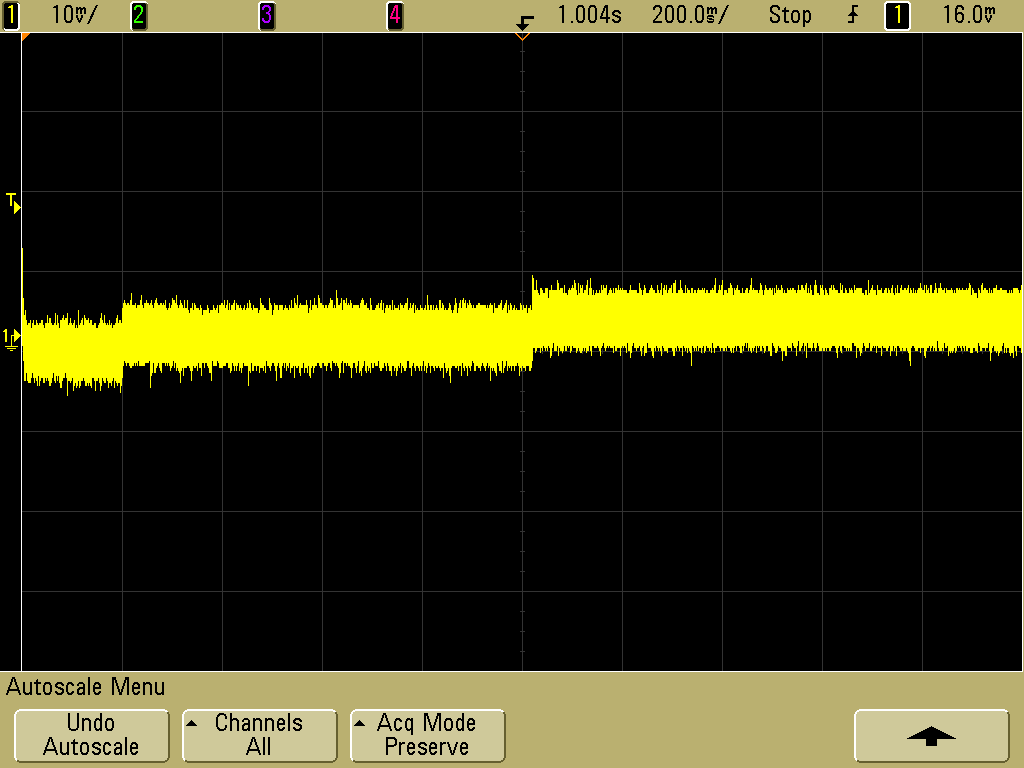
\includegraphics[width=0.7\linewidth]{pics/print_000.png}}
  \caption{Initial two second measurement.}
  \label{fig00}
\end{figure}
\begin{figure} \centering{
  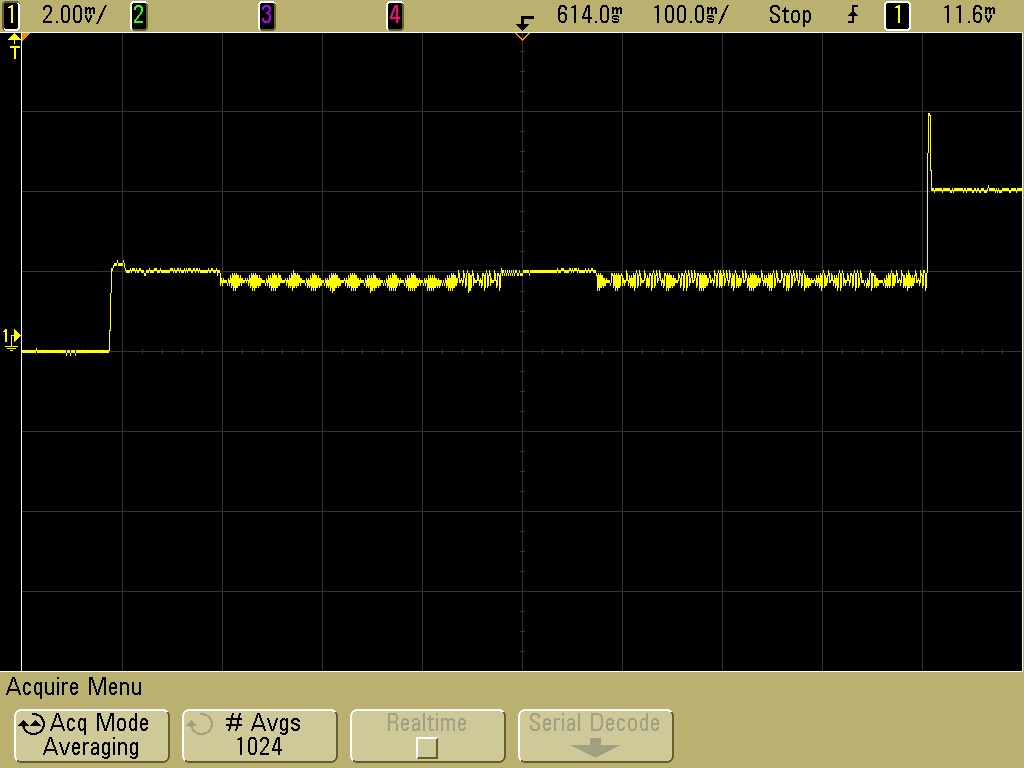
\includegraphics[width=0.7\linewidth]{pics/print_001.png}}
  \caption{Two second measurement cleaned up via averaging.}
  \label{fig01}
\end{figure}
\begin{figure} \centering{
  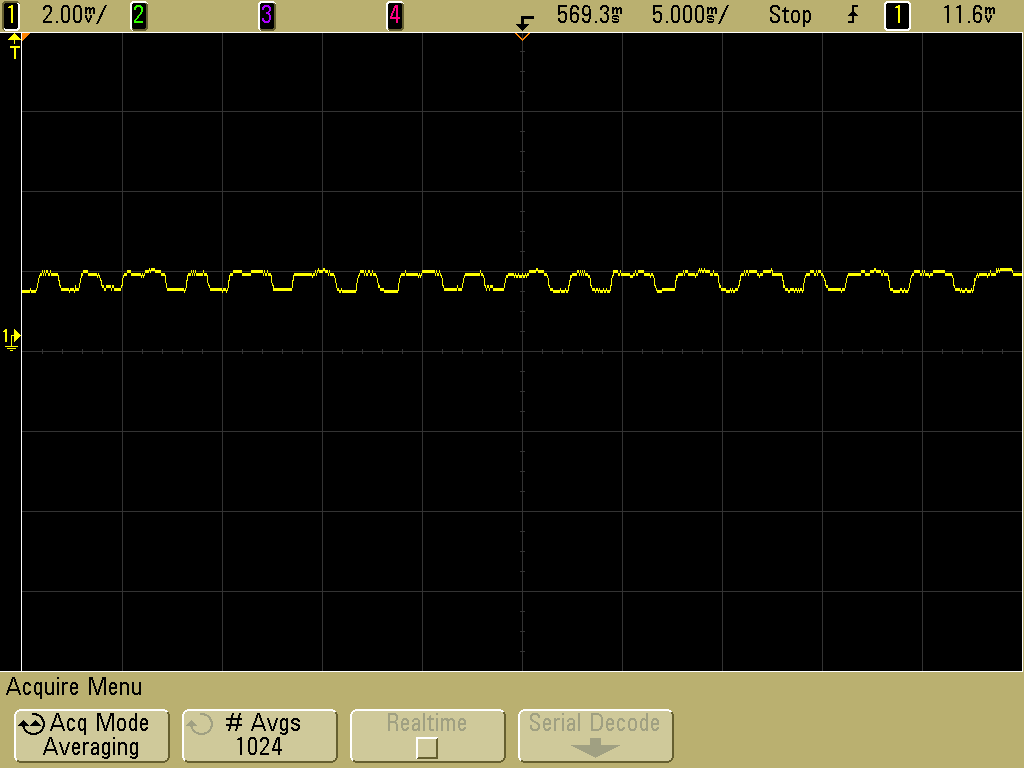
\includegraphics[width=0.7\linewidth]{pics/print_002.png}}
  \caption{LSBs of the public exponent.}
  \label{fig02}
\end{figure}
\begin{figure} \centering{
  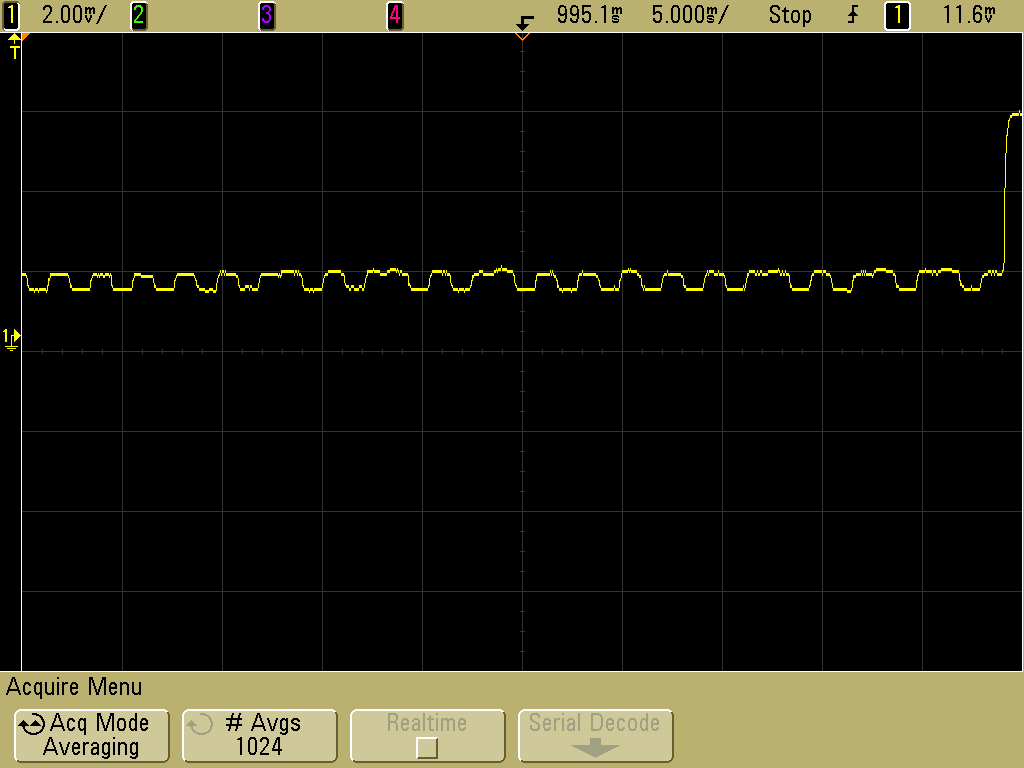
\includegraphics[width=0.7\linewidth]{pics/print_003.png}}
  \caption{LSBs of the private exponent.}
  \label{fig03}
\end{figure}

\end{document}
